\subsection{Спектральные классификация звёзд}
Звёзды в зависимости от формы своего спектра делятся на \imp{спектральные классы}, основные из них представлены в Таблице \ref{tab:spectr-types}. Данная классификация называется Гарвардской и основывается на линиях, которые четко связаны с температурой звезды. Масса, радиус и светимость приведены средних представителей спектрального класса, лежащих на главной последовательности (V).

\begin{table}[h!]
    \centering
    \footnotesize
    \renewcommand{\arraystretch}{1.4}
    \renewcommand{\tabcolsep}{0pt}
    \begin{tabularx}{\tw}{|C{0.1}|C{0.3}|C{0.23}|C{0.13}|C{0.13}|C{0.13}|}
        \hline
        {\bfseries Класс} & {$\mathbf{T}$, К} & {\bfseries Цвет} & {$\mathbf{M}$, $M_{\odot}$} & {$\mathbf{R}$, $R_{\odot}$} & {$\mathbf{L}$, $L_{\odot}$}\\
        \hline
        O & $3 \times 10^4$ --- $6 \times 10^4$ & Голубой & 60 & 15 & $1.4 \times 10^6$\\

        B & $1 \times 10^4$ --- $3 \times 10^4$ & Бело-голубой & 18 & 7 & $2 \times 10^4$\\

        A & $7.5 \times 10^3$ --- $1 \times 10^4$ & Белый & 3.1 & 2.1 & 80\\

        F & $6 \times 10^3$ --- $7.5 \times 10^3$ & Жёлто-белый & 1.7 & 1.3 & 6\\

        G & $5 \times 10^3$ --- $6 \times 10^3$ & Жёлтый & 1.1 & 1.1 & 1.2\\

        K & $3.5 \times 10^3$ --- $5 \times 10^3$ & Оранжевый & 0.8 & 0.9 & 0.4\\

        M & $2 \times 10^3$ --- $3.5 \times 10^3$ & Красный & 0.3 & 0.4 & 0.04\\
        \hline
    \end{tabularx}
    \caption{Гарвардская спектральная классификация звёзд}
    \label{tab:spectr-types}
\end{table}

Внутри каждого спектрального класса выделяют 10 подклассов от 0 до 9, иногда используется десятичная запись (например K4.5). Подклассы в начале последовательности называются ранними, а те, что в конце — поздними. Данная подклассификация говорит только о положении на прямой спектральных классов, она связана с температурой звезды сложным образом — функция перехода от номера подкласса к температуре не является ни строго линейной, ни строго логарифмической, а также является разной для разных спектральных классов.

Ниже приведён график зависимости интенсивности линий от спектрального класса \picRef{pic:lines}, а также список основных линий внутри каждого из них:

\begin{itemize}
	\item \term{Класс O}. Спектр в основном состоит из линий  многократно ионизованных атомов, видны линии гелия, линии водорода слабые.
	\item \term{Класс B}. Отсутствуют линии He$\,$II, линии He$\,$I (4030$\,\mathring{\text{A}}$) наиболее интенсивны в B2 и пропадают к B9. Сильнее проявляются линии водорода, а также становится заметным характерный горб в районе бальмеровского скачка.
	\item \term{Класс A}. Очень сильные линии водорода, полностью пропадают линии гелия.
	\item \term{Класс F}. Ослабевают линии водорода, начинают появляться линии других металлов. 
	\item \term{Класс G}. Продолжают слабеть линии водорода. Линии натрия (3934$\,\mathring{\text{A}}$ и 3968$\,\mathring{\text{A}}$) достигают максимума интенсивности в G0.
	\item \term{Класс K}. Доминируют линии металлов. Линии водорода уже незаметны, линии натрия хорошо видны. В K5 и далее начинают наблюдаться линии оксида титана.
	\item \term{Класс M}. Становятся сильнее линии оксида титана, очень много линий нейтральных металлов.
\end{itemize}

\begin{figure}[h!]
	\centering
	\tikzsetnextfilename{lines}
	\begin{tikzpicture}
		\begin{axis} [
                width   =    \tw,
                height  =    6cm,
                xmax    =    1,
                xmin    =    0,
                ymax    =    0.7,
                ymin    =    0,
                xtick={0.106, 0.236, 0.394, 0.547, 0.705, 0.855},
                ytick=\empty,
                scaled ticks=false,
                xticklabels={B0, A0, F0, G0, K0, M0},
%                extra x ticks={0.106, 0.236, 0.394, 0.547, 0.705, 0.855}, 
%    			extra x tick labels={30000, 10000, 7500, 6000, 5000, 3500}, 
%    			extra x tick style={xticklabel pos=top},
    			ylabel  =	{Относительная интенсивность},
    			grid		=	none,
    			ylabel style={at={(rel axis cs:-0.02,0.5)}}
            ]
				\addplot[black, smooth, thin, dashed] table[col sep=comma] {data/lines-He-II.csv} node at (rel axis cs:0.03, 0.7) {\scriptsize{He II}};
				\addplot[black, smooth, thin, dashed] table[col sep=comma] {data/lines-Si-IV.csv} node at (rel axis cs:0.07, 0.38) {\scriptsize{Si IV}};
				\addplot[black, smooth, thin] table[col sep=comma] {data/lines-He-I.csv} node at (rel axis cs:0.11, 0.7) {\scriptsize{He I}};
				\addplot[black, smooth, thin, dashed] table[col sep=comma] {data/lines-Si-III.csv} node at (rel axis cs:0.12, 0.3) {\scriptsize{Si III}};
				\addplot[black, smooth, thin, dashed] table[col sep=comma] {data/lines-Si-II.csv} node at (rel axis cs:0.24, 0.26) {\scriptsize{Si II}};
				\addplot[black, smooth, thin, dashed] table[col sep=comma] {data/lines-Mg-II.csv} node at (rel axis cs:0.25, 0.42) {\scriptsize{Mg II}};
				\addplot[black, smooth] table[col sep=comma] {data/lines-H-I.csv} node at (rel axis cs:0.27, 0.87) {\scriptsize{H I}};
				\addplot[black, smooth, thin] table[col sep=comma] {data/lines-Fe-II.csv} node at (rel axis cs:0.6, 0.43) {\scriptsize{Fe II}};
				\addplot[black, smooth, dashed] table[col sep=comma] {data/lines-Ca-II.csv} node at (rel axis cs:0.73, 0.77) {\scriptsize{Ca II}};
				\addplot[black, smooth, thin, dashed] table[col sep=comma] {data/lines-Fe-I.csv} node at (rel axis cs:0.77, 0.42) {\scriptsize{Fe I}};
				\addplot[black, smooth, thin] table[col sep=comma] {data/lines-Ca-I.csv} node at (rel axis cs:0.85, 0.5) {\scriptsize{Ca I}};
				\addplot[black, smooth, dashed] table[col sep=comma] {data/lines-Ti-O.csv} node at (rel axis cs:0.93, 0.77) {\scriptsize{Ti O}};
            \end{axis}
	\end{tikzpicture}
	\caption{Относительная интенсивность основных линий}
    \label{pic:lines}
\end{figure}

Помимо основных спектральных классов звёзд существуют дополнительные: W — звёзды Вольфа-Райе, очень тяжёлые яркие звёзды с температурой порядка 70000 К и интенсивными эмиссионными линиями спектра; L — звёзды или коричневые карлики с температурой 1500–2000 К и соединениями металлов в атмосфере; T — метановые коричневые карлики с температурой 700-1500 К; Y — очень холодные (метано-аммиачные) коричневые карлики с температурой ниже 700 К; C — углеродные звёзды, гиганты с повышенным содержанием углерода. Ранее относились к классам R и N.

Однако гарвардская классификация учитывает лишь влияние температуры на спектр, для более точного разбиения вместе с температурой требуется учитывать и светимость звезды. Классификация звёзд по светимости называется Йеркской и основывается она на линиях, которые напрямую связаны с силой гравитации на поверхности звезды. Классификация сводится к разбиению на 6 классов:
\begin{itemize}
	\item \term{Класс Ia}. Наиболее яркие свехргиганты;
	\item \term{Класс Ib}. Менее яркие сверхгиганты;
	\item \term{Класс II}. Яркие гиганты;
	\item \term{Класс III}. Гиганты;
	\item \term{Класс IV}. Субгиганты;
	\item \term{Класс V}. Звёзды главной последовательности (карлики);
	\item \term{Класс VI}. Субкарлики;
	\item \term{Класс VII}. Белые карлики.
\end{itemize}
Запись спектрального класса представляет собой латинскую букву, арабское число и римское число, например, спектральный класс Солнца — G2V. Спектральный класс (показатель цвета) и абсолютная звёздная величина задают положение звезды на \imp{Диаграмме Герцшпрунга-Рассела}. Ниже приведены примеры спектров звёзд разных спектральных классов внутри класса светимости V \picRef{pic:stellar-spectra}.
\begin{figure}[h!]
	\centering
	\foreach \x/\lege in {spectrum_O9V/O9V, spectrum_B8V/B8V, spectrum_A0V/A0V, spectrum_F0V/F0V, spectrum_G0V/G0V, spectrum_K3V/K3V} {
    \begin{subcaptionblock}{\tw}
        \tikzsetnextfilename{\x}
        \begin{tikzpicture}
            \begin{axis} [
                width   =    \tw,
                height  =    3.5cm,
                xmax    =    10000,
                xmin    =    1000,
                scaled ticks=false,
                xticklabel=\empty,
                grid=both,
                legend cell align=left,
            	legend style={
                row sep = 0.8pc,
                draw=none,
                fill=none,
                font=\scriptsize,
                at={(axis cs:9000, 1)}, anchor=north west,
            	}
            ]
                \addplot[black, smooth] table[col sep=comma, x=wavelength, y=spectrum] {data/\x.csv};
            \end{axis}
            \node[anchor=north east] at (rel axis cs: 0.99, 1) {\scriptsize\lege};
    \end{tikzpicture}
    \end{subcaptionblock}
    \hspace{-0.5cm}
  	\hfill
    }
    \begin{subcaptionblock}{\tw}
        \tikzsetnextfilename{spectrum-M0V}
        \begin{tikzpicture}
            \begin{axis} [
                width   =    \tw,
                height  =    3.5cm,
                xmax    =    10000,
                xmin    =    1000,
                scaled ticks=false,
                xtick={1000, 2000, 3000, 4000, 5000, 6000, 7000, 8000, 9000, 10000},
                xlabel  =    {Длина волны $\lambda,~\,\mathring{\text{A}}$},
                grid=both,
                legend cell align=left,
            	legend style={
                row sep = 0.8pc,
                draw=none,
                fill=none,
                font=\scriptsize,
                at={(axis cs:9000, 0.25)}, anchor=north west,
            	}
            ]
                \addplot[black, smooth] table[col sep=comma, x=wavelength, y=spectrum] {data/spectrum_M0V.csv};
            \end{axis}
            \node[anchor=north east] at (rel axis cs: 0.99, 0.37) {\scriptsize M0V};
    \end{tikzpicture}
    \end{subcaptionblock}
    \caption{Спектры звёзд}
    \label{pic:stellar-spectra}
\end{figure}


%    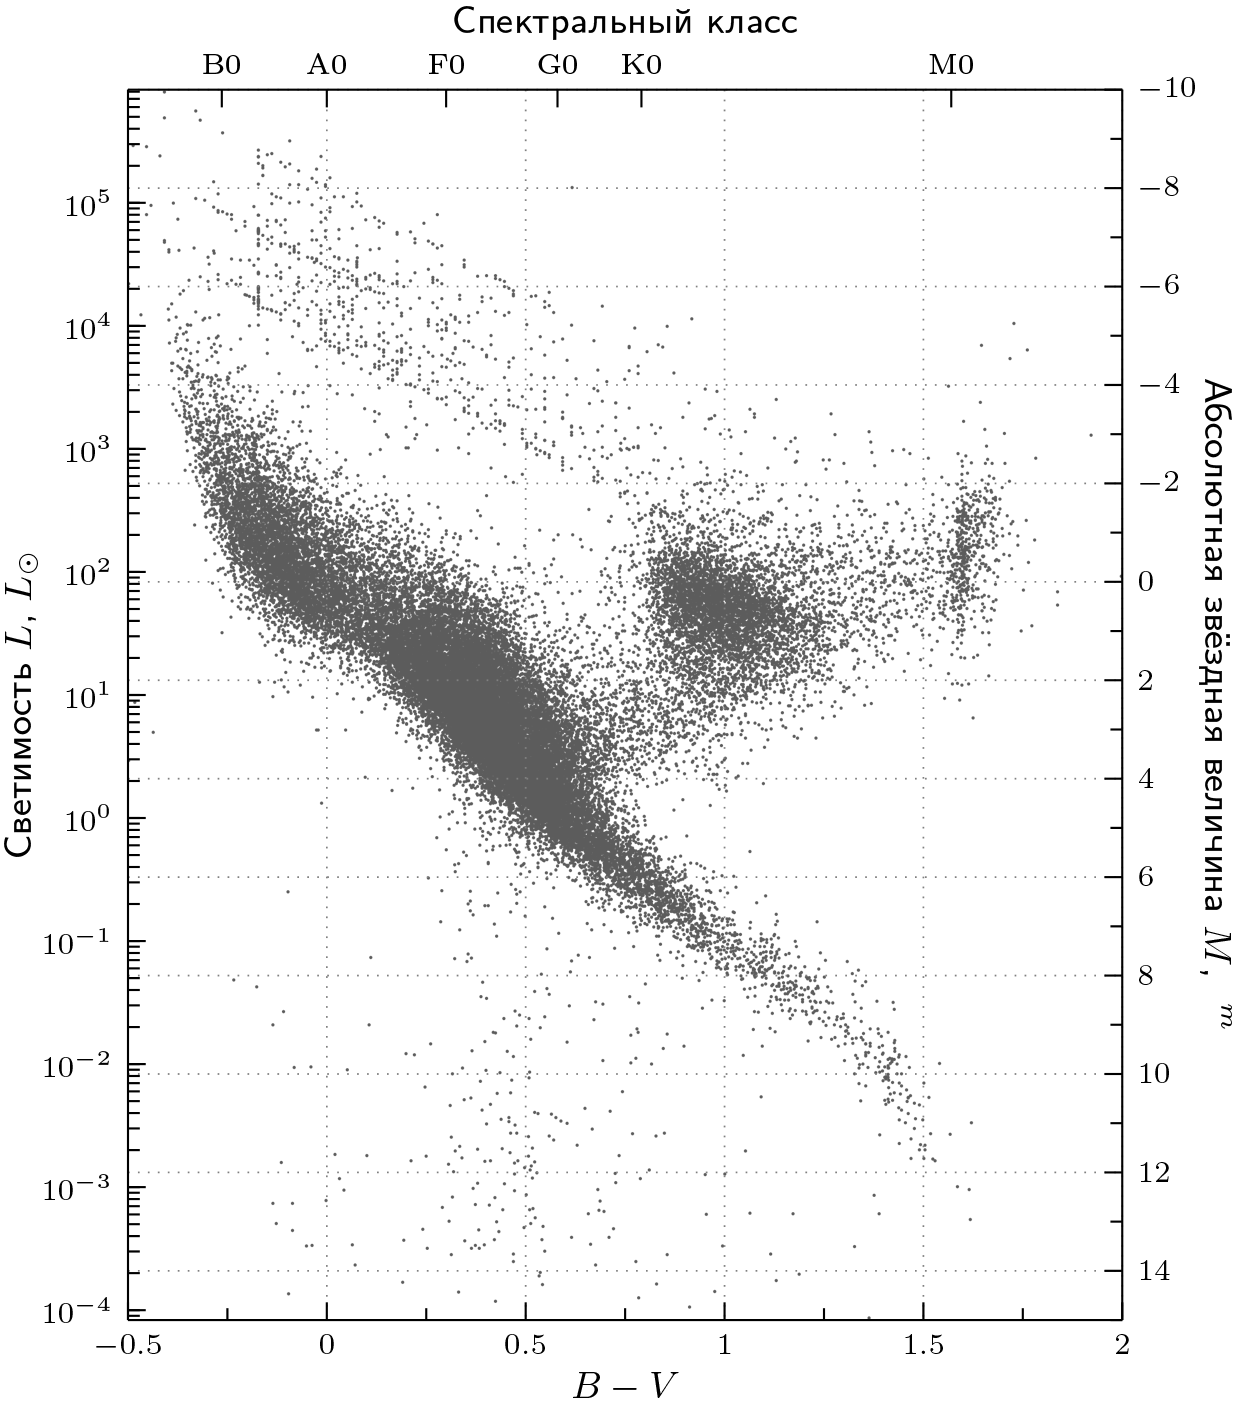
\includegraphics[width=10cm]{gr}

\term{Диаграмма Герцшпрунга-Рассела} показывает зависимость светимости или абсолютной звёздной величины от спектрального класса, показателя цвета $(B-V)$ или эффективной температуры фотосферы звезды.

Была предложена примерно в 1910 году независимо Эйнаром Герцшпрунгом и Генри Расселом. Диаграмма используется для классификации звёзд и соответствует современным представлениям о звёздной эволюции.

Около $90 \%$ звёзд находятся на главной последовательности. Их светимость обусловлена термоядерными реакциями превращения водорода в гелий. Выделяется также несколько ветвей проэволюционировавших звёзд-гигантов, в которых происходит горение гелия и более тяжёлых элементов. В левой нижней части диаграммы находятся полностью проэволюционировавшие белые карлики.

Мнемонические правила для запоминания спектральных классов: <<\textbf{O}h \textbf{B}e \textbf{A} \textbf{F}ine \textbf{G}irl, \textbf{K}iss \textbf{M}e \textbf{R}ight \textbf{N}ow \textbf{S}weetheart.>> и <<\textbf{В}ообразите: \textbf{О}дин \textbf{Б}ритый \textbf{А}нгличанин \textbf{Ф}иники \textbf{Ж}евал \textbf{К}ак \textbf{М}орковь --- \textbf{Р}азве \textbf{Н}е \textbf{С}мешно?>>
\begin{figure}[h!]
    \centering
    \vspace{-1pc}
    \tikzsetnextfilename{hr-diagram}
    \begin{tikzpicture}
         \begin{axis}[
                         height    =    10cm,
                         width    =    10cm,
                         ymax    =    14.,
                         ymin    =    -6.,
                         y dir    =    reverse,
                         xmax    =    2.,
                         xmin    =    -.5,
                         axis x line* = bottom,
                         axis y line* = right,
                         xlabel  =   $B-V$,
                         y label style = {at={(axis description cs: 1.07, 0.5)}, rotate=180},
                         ylabel    =    {Абсолютная звёздная величина $M$, $\!~^m$}
                     ]
            \ifthenelse{\boolean{useLightPlotVersion}}{}{
                \addplot+[only marks, mark = o, mark options={scale=0.2, darkgray}] table[x=BV, y=M, col sep = comma]{data/gr-plot.csv};
            }
         \end{axis}
         \begin{semilogyaxis}[
                         height    =    10cm,
                         width    =    10cm,
                         ymax    =    2.088e4,
                         ymin    =    2.088e-4,
                         xmax    =    2.,
                         xmin    =    -.5,
                         minor x tick num = 0,
                         minor y tick num = 01,
                         xtick = {-0.264, 0, 0.3, 0.58, 0.791, 1.57},
                         xticklabels = {B0, A0, F0, G0, K0, M0},
                         axis x line* = top,
                         axis y line* = left,
                         xlabel    =    {Спектральный класс},
                         x label style = {at={(axis description cs: 0.5, 1.03)}, rotate=0},
                         ylabel    =    {Светимость $L$, $L_\odot$},
                         ymajorgrids     =    false,
                         xmajorgrids     =    false
                    ]
        \end{semilogyaxis}
     \end{tikzpicture}
     \caption{Диаграмма Герцшпрунга--Рассела}
    \label{}
\end{figure}

\term{Линии Фраунгофера} — линии поглощения в спектре Солнца подробно описанные Йозефом Фраунгофером в 19 веке. Наиболее яркие среди них называются латинскими буквами от A до K и упорядочены в порядке \imp{уменьшения длины волны} см. Таблицу\,\ref{tab:fraunhofer-lines}.
\begin{table}[h!]
    \centering
    \footnotesize
    \renewcommand{\arraystretch}{1.4}
    \renewcommand{\tabcolsep}{0pt}
    \begin{tabularx}{0.55\tw}{|C{0.36}|C{0.22}|C{0.42}|}
        \hline
        {\bfseries Обозначение} & {\bfseries Элемент} & {\bfseries Длина волны, $\mathring{\text{A}}$} \\
        \hline
        A & $\text{O}_2$ & 7594\\

        B & $\text{O}_2$ & 6867\\

        C & $\text{H}_\alpha$ & 6563\\

        $\text{D}_{12}$ & Na & 5896, 5890\\

        F & $\text{H}_{\beta}$ & 4958\\

        G' & $\text{H}_{\gamma}$ & 4340\\

        H & Na & 3968\\
        
        K & Na & 3934\\
        \hline
    \end{tabularx}
    \caption{Линии Фраунгофера}
    \label{tab:fraunhofer-lines}
\end{table}










